\documentclass[10pt]{exam}
\usepackage[icp]{template-for-exam}
\usepackage{tikz}
\usetikzlibrary{patterns}


%\printanswers
\shadedsolutions



\newcommand{\printeqs}{
  \ifprintanswers
  \else
    \begin{center}
      \begin{tabular}{|*9c*5c|}
        \hline 
        &&&&&&&&&&&&&\\
        && 
        $W=Fd$                 & & & 
        $KE = \frac{1}{2}mv^2$ & & & 
        $PE=mgh$               & & & 
        $g=\SI{9.8}{\meter\per\second^2}$
        &&\\
        &&&&&&&&&&&&&\\
        \hline 
      \end{tabular}
    \end{center}
  \fi
}

\newenvironment{EnvKU}{
  \ifprintanswers
  \else
    \ku
  \fi
  \begin{solution}
}{
  \end{solution}
}


\title{Unit P4 Review (Energy)}
\author{Rohrbach}
\date{\today}

\begin{document}
\maketitle

\printeqs 
\begin{questions}
  
 
\question
  Define the following terms

  \begin{parts}
    \item work
      \begin{solution}[\stretch{1}]
        the product of force and distance
      \end{solution}

    \item energy
      \begin{solution}[\stretch{1}]
        the ability to do work
      \end{solution}

    \item kinetic energy
      \begin{solution}[\stretch{1}]
        energy due to motion
      \end{solution}

    \item potential energy
      \begin{solution}[\stretch{1}]
        energy that is stored
      \end{solution}

  \end{parts}

\question
  What are the units for energy?
  
  \begin{solution}[\stretch{1}]
    Joules (J)
  \end{solution}


\question
  What are the four types of {\bf potential energy}?

  \begin{solution}[\stretch{1}]
    elastic, gravitational, nuclear, chemical
  \end{solution}


\question
  Calculate the work done if 5 N of force is used to push a grocery cart 3 m. 

  \begin{EnvKU}
    \begin{align*}
      F &= \SI{5}{\newton} & W &= Fd \\
      d &= \SI{3}{\meter}  & W &=(5)(3) \\
      W &= \text{?}            & W &= \SI{15}{\joule}
    \end{align*}
  \end{EnvKU}

\pagebreak

\printeqs

\question
  What is the kinetic energy of the wrecking ball with a mass of 200 kg if it swings with a velocity of 15 m/s?

  \begin{EnvKU}
    \begin{align*}
      m  &= \SI{200}{\kilo\gram}
                          & KE &= \frac{1}{2}mv^2 \\
      v  &= \SI{15}{\meter\per\second}    
                          & KE &= \frac{1}{2}(200)(15)^2 \\
      KE &= \text{?}
                          & KE &= (0.5)(200)(225) \\
         &                & KE &= \SI{22500}{\joule}
    \end{align*}
  \end{EnvKU}

\question
  What two things are needed in order for work to be done?

  \begin{solution}[\stretch{1}]
    force and distance
  \end{solution}

\question
  Decide if work is being done in each of the following situations.  Explain.

  \begin{parts}
    \item 
      You push very hard against a stationary wall.
    
      \begin{solution}[3em]
        no, there is no distance
      \end{solution}

    \item 
      When the light turns green, a car accelerates forward for three blocks.
    
      \begin{solution}[3em]
        yes, there is a force, and the car is moving a distance.
      \end{solution}

    \item 
      A woman holds a child on her shoulders to watch a parade.
    
      \begin{solution}[3em]
        no, the child is not moving a distance
      \end{solution}

    \item
      A woman lifts a child to her shoulders.
    
      \begin{solution}[3em]
        yes, there is a force, and the car is moving a distance.
      \end{solution}

  \end{parts}

\question
  Explain what the term ``energy is conserved'' means.

  \begin{solution}[\stretch{1}]
    the total energy of a system does not change.
  \end{solution}

\question
  When does an object have zero kinetic energy? 

  \begin{solution}[3em]
    when it is not moving
  \end{solution}

\question
  When does an object have zero gravitational potential energy?

  \begin{solution}[3em]
    when it is on the ground
  \end{solution}

\pagebreak
\printeqs

\question
  You drop a ball.  Explain what kinds of energy it has in each of the following cases:

  \begin{parts}
    \item 
      Before it falls (while it's still in your hand)

        \begin{solution}[3em]
          all energy is PE
        \end{solution}

    \item 
      While it is falling

        \begin{solution}[3em]
          PE is decreasing; KE is increasing
        \end{solution}

    \item 
      Just before it hits the ground

        \begin{solution}[3em]
          all energy is KE
        \end{solution}

  \end{parts}


\question
  Fill in the missing kinetic energy values for the following marble rolling down a ramp:


  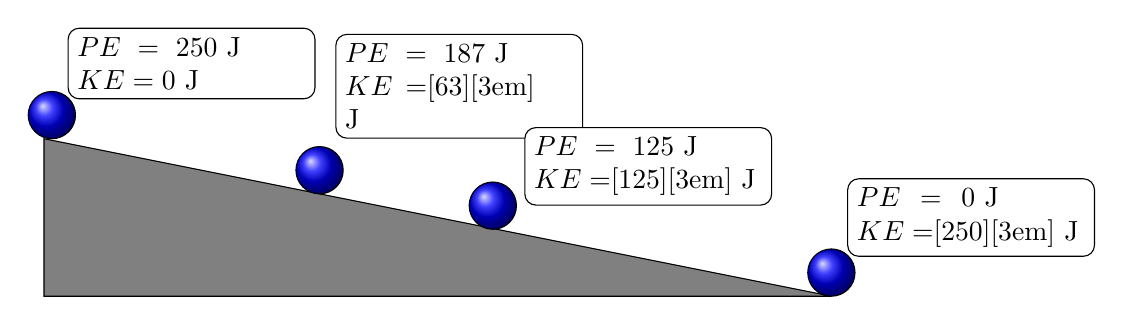
\begin{tikzpicture}
    \tikzset{
      ball/.append style={
        shading=ball,
        minimum width=15pt
      },
      ennode/.append style={
        text width=2.9cm,
        anchor = south west,
        fill = white,
        rounded corners,
        draw = black,
      }
    }
    \filldraw[fill=gray] (0,0) -- (0,2) -- (10,0) -- cycle;
    \draw[ball] (.1,2.3) circle (0.3) coordinate (a);
   \draw[ball] (3.5,1.6) circle (0.3) coordinate (b);
    \draw[ball] (5.7,1.15) circle (0.3) coordinate (c);    \draw[ball] (10,.3) circle (0.3) coordinate (d);
    \draw (a) + (.2,.2) node[ennode] 
      {$PE=250$ J \hspace{\stretch{1}} $KE=0$ J};
    \draw (b) + (.2,.4)  node[ennode] 
      {$PE=187$ J \hspace{\stretch{1}} $KE=$\fillin[63][3em] J};
    \draw (c) + (.4,0) node[ennode] 
      {$PE=125$ J \hspace{\stretch{1}}  $KE=$\fillin[125][3em] J};
    \draw (d) + (.2,.2) node[ennode] 
      {$PE=0$ J \hspace{\stretch{1}} $KE=$\fillin[250][3em] J };
  \end{tikzpicture}

\question
  What is the gravitational potential energy of a wrecking ball that is hung 20 meters above ground if it has a mass of 200 kg?  

  \begin{EnvKU}
    \begin{align*}
      m  &= \SI{200}{\kilo\gram}
                                & PE &= mgh \\
      g  &= \SI{9.8}{\meter\per\second^2}    
                                & PE &= (200)(9.8)(20) \\
      h  &= \SI{20}{\meter}    \\
      PE &= \text{?}
                                & PE &= \SI{39200}{\joule}
    \end{align*}
  \end{EnvKU}


\question
  A force of 13 N is applied on a cart.  If 125 J of work is done, how far did you push the cart?

  \begin{EnvKU}
    \begin{align*}
      F  &= \SI{13}{\newton} &  W                &= Fd    \\
      W  &= \SI{125}{\joule} & 125               &= (13)d \\
      d  &= \text{?}         & \SI{9.62}{\meter} &= d
    \end{align*}
  \end{EnvKU}

\end{questions}

\ifprintanswers
\else
  \pagebreak
  \hfill
\fi

\end{document}